% SCIS 2018 English manuscript (for LaTeX2e)
\documentclass[a4paper]{article}
\usepackage{Style}
\usepackage{graphics, graphicx}
\usepackage{enumitem}
\usepackage{color}
% If you use LaTeX 2.09, delete the above two lines and remove '%' below.
%\documentstyle[scis2018e]{jarticle}

\begin{document}

\title{
  Title of This Paper     %The title of this paper
}
\author{
  First Author           %The name of the first author
  \thanks{
    Affiliation1, Address1,   %The affiliation and address of the first author
    (E-mail addresses are placed here if you like.)
  }
  \and
  Second Author          %The name of the second author
  \thanks{ %If this is same as the first author, write \samethanks{1}.
    Affiliation2, Address2  %The affiliation and address of the second author
  }
}
\abstract{
  In this paper ....  % Abstract of this paper
}
\keywords{
  keyword1, keyword2, ... %Index terms of this paper
}

\maketitle

\section{The First Section}

The contents of the first section.

\newpage
.
\newpage
\section{Background}
In this section, we are going to briefly explain various materials that we would cover for our attacks. Including variants of the cache attacks we are going to discuss upon attacking the block ciphers, and also some ideas about the searchable encryption.

\subsection{Cache Attacks}

The cache attacks are one of the side channel attacks that is able to recover information about AES T-table or AES key, for even better case. There are 2 most prominent attack, which are called $PRIME+PROBE$ and $FLUSH+RELOAD$.

\subsubsection{PRIME+PROBE}

$PRIME+PROBE$ attacks first loads and occupies a cache set, a set of cache lines, with some dummy code. Then after some moment, measure the time reading data that were loaded on the target cache set. If there was any cache eviction by another process, which in this context the victim, loading would take longer duration as cache miss would occur. This attack doesn't need a shared memory between target and the hostile, but the lowest unit it can attack as a whole set.

\subsubsection{FLUSH+RELOAD}

$FLUSH+RELOAD$ attacks relies upon the inclusive property of the cache policy that is held by the Intel chips. The inclusive property of the cache is that everything on L1 cache should be also on L3 cache. Thus, whenever a cache line is loaded on L1 cache, they are also loaded on L3 cache. Likewise, when a CLFLUSH, or cache flush is called for a cache line within L1 cache, then the same line is evicted from L3 cache.\par
The basic idea of $FLUSH+RELOAD$ is both victim core and the attacker's core load same line of data or instruction from the shared memory. Then the attacker flush the shared cache line from its core. Flushed from the L1 cache, the same line is evicted from L3 cache, and also evicted from the victim's L1 cache as a cascade. Now what we have to observe is that whenever victim cache reloads the same line onto its cache, the very same line is loaded onto the L3 cache again. Meaning that when the attacker reloads the line, the reload time is shortened. This attack obviously need a shared memory between the victim and the attacker, but as an opposite to the $PRIME+PROBE$ attack, it can attack as small as a single line, giving more granuality on the attack.

\subsection{SSL/TLS}
Secure Sockets Layer (SSL) is a kind of Internet Protocol (IP) for communication on Internet. SSL was developed by Netscape Corporation in 1993. The goal of this protocol is that overcome the problem of no confidentiality. SSL ver3.0 is standardized in Internet Engineering Task Force (IETF) and re-named Transport Layer Security (TLS).

Standardized TLS \cite{TLS1, TLS2} ensures secure connection between a server and a client. This protocol uses records as a fundamental unit in communication. With these records, the server and the client initiates handshake protocol, where they negotiate the cipher they will use to encrypt the application itself and exchange the master key used for the encryption. Therefore, TLS provides effective functions such as identity verification, message integrity, and confidentiality.

Although this protocol (TLS 1.2) is used as a standard in Internet, it had various vulnerabilities, either from its structure or implementation, which led many different attacks to threat the secrecy, including timing attacks or heartbleed attacks that we are going to discuss later. To deal these attacks, TLS 1.3 drafts are currently developed and some of them are in use nowadays. Amongst those, most commonly used method is to build a tunnel through SSL channel, where the traffic from the user is encrypted using either SSL or TSL protocol. By using already secure channel that is implemented in web browsers, this method allows users to access to their web browsers simply.

\subsection{Key Exchange}
The secret key is no longer meaningful when both parties exchange their secret keys publicly.
Therefore, they need to hide each other's secret keys from others. Key exchange is a method for secure communication satisfying this condition between each other. Therefore, the shared key must be known only to the sender and the receiver, and they should be able to check whether each other is the one with which they want to communicate. If an attacker intercepts data in the middle, the attacker must not be able to retrieve the value of the shared key from the data.

\subsection{Diffie–Hellman Key Exchange}
Diffie-Hellman key exchange \cite{diffie} is one way to exchange cryptographic keys, allowing two people to share a common secret key over an unencrypted network. Diffie and Hellman published it in 1976. Diffie-Hellman key exchange has established a basic cryptographic communication method and is still in use today. In 1977, RSA encryption, a public key cryptosystem, was proposed. Diffie-Hellman key exchange is performed as follows.
\begin{enumerate}[label=]
      \item 1) First, Alice chooses a prime $p$ and an integer $g$ from 1 to $p-1$ and shares it with Bob in advance. 
      
      \item 2) Alice selects integer $a$. This integer is not disclosed to the outside, and Bob is also unknown.
      
      \item 3) Alice calculates $A = g^{a}\ mod\ p$
      \item 4) Bob also selects integer b and calculates $B = g^{b}\ mod\ p$
      \item 5) Alice and Bob send $A$ and $B$ to each other
      \item 6) Alice calculates $B^{a}\ mod\ p$ and Bob calculates $A^{b}\ mod\ p$
      \item 7) $B^a\ mod\ p = (g^b)^a\ mod\ p = g^{ab}\ mod\ p$ and $A^b\ mod\ p = (g^a)^b\ mod\ p = g^{ab}\ mod\ p$
      \item 8) Finally, Alice and Bob share a common secret key of $g^{ab}\ mod\ p$
\end{enumerate}
Here, if $p$ is sufficiently large, an attacker who wants to know the secret key from the outside can not calculate the secret key, so that secure key exchange becomes possible.


\subsection {RSA cryptosystem}
RSA is a asymmetric key cryptosystem proposed by Rivest, Shamir, and Adleman [35Ms]. This system has public key and private key. RSA Scheme is defined as follows:

\textbf{Key Generation}
\begin{enumerate}[label=]
      \item 1) Select two large primes $p$, $q$.
      
      \item 2) Compute modulus $n=pq$, and $\phi(n)$ 
      
      \item 3) Pick an integer \textit{e} relatively prime to $\phi(n)$, i.e. gcd($e$,$\phi(n)$))=1
      
      \item 4) Compute $d$ such that $ed$=1 (mod ($\phi(n)$)
      
      \item 5) Set ($n$,$e$) as public key  and ($p$,$q$,$d$) as secret key  
\end{enumerate}

\textbf{Encryption}
\begin{enumerate}[label=]
      \item 1) ciphertext $C$ is computed by  $C \equiv M^e \ (mod \ n)$ where $M$ is plaintext
\end{enumerate} 

\textbf{Decryption}
\begin{enumerate}[label=]
      \item 1) Compute $M' \equiv C^d \ (mod \ n)$ where $M'$ is recovered plaintext
      \item 2) Check whether $M=M'$
\end{enumerate} 

Security of RSA is relied on hardness of Interger Factorization Problem(IFP). If we want to recover plaintext from ciphertext, we should know $p$ or $q$ or $d$. It is computationally infeasible to factorize 1024-bit (or larger) key $n$ with general algorithms such as the number field sieve (NFS) or the older quadratic sieve (MPQS). Thus if we correctly generate $p$ and $q$, then security of RSA is guaranteed.

\subsection{Digital Signature Algorithm(DSA)}
DSA is a Federal Information Processing Standard for digital signatures. This scheme is a variant of ElGamal signature scheme. Details of scheme is described as follows:
\\

\textbf{Parameters}: Let $H$ be a collision-resistant hash function. Let $q$ be a large prime (usually, 160 bits are used). Choose prime number $p$ such that $q$ divides $q-1$. Let $g<p$ be a primitive element of $Z_p^*$
\\

\textbf{Key Generation}
\begin{enumerate}[label=]
      \item 1) Choose a secret key $x$ randomly with $0<x<q$
      
      \item 2) Compute $y \equiv g^x$ (mod $p$)
      
      \item 3) Public key is $y$; long-term secret key is $x$
\end{enumerate}

\textbf{Signature Generation}
\begin{enumerate}[label=]
      \item 1) Choose a random ephemeral secret $k$ such that $0<k<q$
      
      \item 2) Compute $r \equiv (g^k$ mod $p$) mod $q$
      
      \item 3) Compute $s \equiv (H(m)+xr)k^{-1}$ (mod $q$)
      
      \item 4) The signature is ($r,s$)
\end{enumerate} 

\textbf{Verification}
\begin{enumerate}[label=]
      \item 1) Reject the signature if $0<r<q$ or $0<s<q$ is not satisfied
      \item 2) Compute $\omega = s^{-1}$ mod $q$
      \item 3) Compute $u_1 = H(m) \cdot \omega$ mod $q$
      \item 4) Compute $u_2 = r \cdot \omega$ mod $q$
      \item 5) Compute $v=(g^{u_1} y^{u_2}$ mod $p$) mod $q$
      \item 6) Check whether $v = r$
\end{enumerate} 

Secutify of DSA is relied on hardness of Discrete Logarithm Problem(DLP). If we want to forge signature, we have to know long-term secret key $x$ or ephemeral secret key $k$. Thus it is essential that only verifier knows $x$ and $k$.

\subsection{Coppersmith's Algorithm}
Coppersmith's algorithm [] is devised to find small roots of univariate modular equations. This root finding algorithm is based on the LLL-reduction algorithm by Lenstra, Lenstra, and Lovasz [17]. The main idea is to encode polynomial equations with small solutions as coefficient vectors that have a small Euclidean norm. Coefficient vectors will be found by an application of the LLL-reduction algorithm.
The detail of algorithm is described as follows:

\textbf{Input} : polynomial $f(x)$ of degree $\delta$, modulus $N$ of unknown factorization that is a multiple of $b$, a lower bound $b \geq N^{\beta}$, $\epsilon \leq {1 \over \gamma} \beta$ where $0<\beta \leq 1$
\\

\textbf{Algorithm}
\begin{enumerate}[label=(\roman*)]
      \item Choose $m=\lceil {\beta^2 \over \delta \epsilon} \rceil$ and t = $\lfloor \delta m ({1 \over \beta}-1) \rfloor$. 
      
      Compute the polynomials 
      
      $g_{i,j} (x) = x^j N^i f^{m-i} (x)$ \\ for $i=0,...,m-1$ ,  $j=0,...,\delta-1$
      
      $h_i(x) = x^i f^m (x)$ for $i=0,...,t-1$
      \item Compute the bound $ X= {1 \over 2} \lceil N^{{\beta^2 \over \delta} - \epsilon} \rceil$. Construct the lattice basis $B$, where the basis vectors of $B$ are the coefficient vectors of $g_{i,j}(xX)$ and $h_i(xX)$.
      \item Apply the LLL algorithm to the lattice basis B. Let $v$ be the shortest vector in the LLL reduced basis. The vector $v$ is the coefficient vector of some polynomial $g(xX)$. Construct $g(x)$ from $v$.
      \item Find the set $R$ of all roots of $g(x)$ over the integers using standard methods. For every root $x_0 \in R$ check whether gcd$(N,f(x_0)) \geq N^{\beta}$. If this condition is not satisfied, then remove $x_0$ from $R$.
\end{enumerate} 

\textbf{Output}: Set $R$, where $x_0 \in R$ whenever $f(x_0)=0$ mod $b$ for $|x_0| \leq X$.
\\

This algorithm can be extended to \textit{Howgrave-Graham method} [].

\section{Classification}

\subsection{Symmetric Ciphers and Its Applications}

We now would first introduce several studies about the recent cache related attack, then would also introduce attacks on the searchable encryption. As a notice, these attacks are not developed to solely attack the symmetric ciphers, but are capable in attacking them. For example, the cache attacks doesn't pin point to break the block ciphers, but also is applicable to various privacy breachings such as detecting the mobile touch or swipe, or retrieving RSA keys. Also, the searchable encryption, by itself, can utilize either the symmetic key ciphers or public key ciphers.

\subsubsection{Cache Attacks}

Recent studies on the cache level attacks, such as ARMageddon, are focusing more on either extending pre-existing attack on other platforms such as ARM processors, which may lack some components in launching classic cache attacks, such as $FLUSH+RELOAD$. Other research, $PRIME+ABORT$, focuses on integrating the new hardware features on the cache attacks so that the performance of the attack is improved.

\subsubsection*{ARMageddon}

Our known and famous $FLUSH+RELOAD$ attack was designed to attack the Intel x86 architecture with its cache policy and assembly intact. Meaning that it had the inclusive cache policy with shared cache for all cores in all of its products, an instruction that would easily flush the cache line, and lastly an easy way to time the cache loading. However, ARM core lacks all of those, which in this paper stated as the challenge as ARM architecture has no inclusive cache policy, big.LITTLE makes some of their chips shipped without shared cache, no explicitly known instruction that would flush a cache line flat, and their cache load time is a priviliged instruction.
\par Yet, they successfully tackle these problem by exploiting the cache coherency policy, which loads a cache line from remote CPU if available, and from DRAM if not. This makes them to be able to detect whether the certain line of the cache is loaded on the core other than the attacker's and also independent from the shared cache. Furthermore, they replaced the flushing with a random eviction bringing the idea from the rowhammer attack. Finally, they solved the timing challenge with other instructions such as system call or clock time measuring. This attack made previous $FLUSH+RELOAD$ attack available for ARM architecture, which is widely used in the mobile devices. They were not only able to retrieve the T-Table and the key for AES in openSSL library, but also detect touch or swipe and gather data leaked from ARM TrustZone.

\subsubsection*{PRIME+ABORT}

$PRIME+ABORT$ focuses on integrating new hardware feature for Intel chips, namely Intel TSX. Simply put, Intel TSX is the hardware implementation of transactional memory, which has similar concept to a transaction in the database. Utilizing Intel TSX goes as follows, a transaction of instructions are either completed or aborted in the transactional memory. Among those abortion conditions, there is a rule that aborts a transaction whenever the cache that the transation is currently using is evicted, the transaction is aborted. Using this rule, the attacker would detect the cache eviction right away instead of wating a fixed term and measuing the data read time. Thus, the real attack loads and occupies whole cache set with the transactional memory, which is similar to the $PRIME+PROBE$. Then the attacker waits for the victim to evict the cache. When the victim evicts the cache, then the transaction is aborted right away, letting the attacker know the exact moment the cache is evicted. This attack proves to be more superior to $PRIME+PROBE$ as it doesn't require any kind of timer as eviction is detected right away. Also this attack is much faster and has less noise than the existing one.

\subsubsection{Test}



\subsection{Public Key}

\subsection{DROWN Attack}
Aviram \textit{et al}.\cite{drown} introduced the Decrypting RSA with Obsolete and Weakened eNcryption (DROWN)  Attack at USENIX in 2016. Generally, SSL / TLS-based certificates use public key algorithms such as RSA. Therefore, in SSL / TLS, many public key related attacks and vulnerabilities are found. Figure 1\footnote{https://www.globalsign.com/en/blog/drown-attack-sslv2/} shows recently discovered vulnerabilities in order. In particular DROWN attack is a relatively recent attack. This vulnerability is known to be a problem with SSLv2. So DROWN shows that supporting SSLv2 is a threat to servers and clients. Nevertheless, there are still many servers using SSLv2. SSLv2 has an RSA-based key exchange process called the Pre Master Secret (PMS) and DROWN applies the attack to this part. TLS also supports RSA, but TLS can respond to attacks on encryption and SSLv2 is not.

The basic scenario of DROWN attack is as follows. 
\begin{enumerate}[label=]
      \item 1) The attacker sniffs the encrypted PMS, sends a lot of related values to the server, and attempts to decrypt the PMS.
      
      \item 2) 2) If PMS decryption is successful through this process, it can find the key value exchanged through RSA and decrypt SSL using this key.
\end{enumerate}  

To decrypt a 2048-bit RSA TLS ciphertext, an attacker must observe 1,000 TLS handshakes, initiate 40,000 SSLv2 connections, and perform $2^{50}$ work. Because most people will not buy multiple certificates, TLS and SSLv2 protocols often use the same private key. Therefore, due to a bug in SSLv2, TLS can be easily applied to attacks. The DROWN attack uses this exact method to break encryption. Actually the authors have implemented the attack and can decrypt a TLS 1.2 handshake using 2048-bit RSA in under 8 hours, at a cost of \$440 on Amazon EC2. So SSLv2 is not only weak, but actively harmful to the TLS ecosystem.

It is very important to prevent this attack, because if we are attacked by a DROWN attack, we will give away important information such as user-names and passwords, credit card numbers, emails, instant messages, and sensitive documents. However, contrary to expectations, the way to prevent a DROWN attack is very simple. As mentioned earlier, this attack starts in the SSLv2 key exchange process, so if we do not use SSLv2, we can effectively prevent the attack. Upgrading OpenSSL\footnote{OpenSSL is a cryptographic library used in many server products. For users of OpenSSL, the easiest and recommended solution is to upgrade to a recent OpenSSL version.} is also a good solution. This method \cite{Openssl} is described in detail on the Internet.

\subsection{Logjam Attack}
Adrian \textit{et al}.\cite{logjam} introduced Logjam attack in 2015. Unlike DROWN attacks based on the construction of the SSLv2 protocol, Logjam attacks are based on the underlying construction issues of the TLS protocol. This attack can downgrade the TLS connection from the existing 1024 bits to the 512 bit grade encryption through a Man-In-The-Middle (MITM) attack. Therefore, both Web browsers and mail servers using TLS may be exposed to this vulnerability. In particular, Diffie-Hellman key exchange is a popular cryptographic algorithm that allows Internet protocols to agree on a shared key and negotiate a secure connection. However, this Diffie-Hellman key exchange can be used as a means of Logjam attack. In an MITM attack for this attack, the attacker tries to connect to the server using the \textbf{DHE$\_$EXPORT} cipher suite instead of the client. This can be performed by a fault in the diffie-Hellman key exchange-based TLS protocol. A key that has been reduced to 512 bits due to an MITM attack can be recovered through numerous CPUs.

This problem can also be resolved by updating the version of OpenSSL as well as the DROWN attack. This is because TLS client protection has been added to deny handshake if the Diffie-Hellman parameter is shorter than 768 bits. It is also a good solution to disable the attacking \textbf{DHE$\_$EXPORT} and create a new 2048-bit Diffie-Hellman group.

\subsection{FREAK Attack}
Factoring RSA Export keys (FREAK) attack that was introduced in 2015 is similar to Logjam attack. Both attacks weaken the cryptosystem by reducing the key size to 512 bits. However, FREAK attack is a running-related vulnerability and Logjam attack differs in that it is a vulnerability in the underlying construction of the TLS protocol itself.

\begin{table}[]
\centering
\caption{Recent SSL/TLS Vulnerabilities}
\label{my-label}
\renewcommand{\tabcolsep}{0.7mm}
\begin{tabular}{|c|c|c|c|}
\hline
\textbf{Date}                                             & \textbf{Name}                                                    & \textbf{Vulnerability}                                                                            & \textbf{Mitigation}                                                                                 \\ \hline
\hline
\begin{tabular}[c]{@{}c@{}}September\\  2011\end{tabular} & BEAST                                                            & \begin{tabular}[c]{@{}c@{}}TLS 1.0,\\ earlier \\ protocols \\ result\end{tabular}                 & \begin{tabular}[c]{@{}c@{}}Use only \\ AES-GCM\\  suites supported \\ only in TLS 1.2.\end{tabular} \\ \hline
\begin{tabular}[c]{@{}c@{}}August \\ 2012\end{tabular}    & BREACH                                                           & \begin{tabular}[c]{@{}c@{}}Leaks \\ plaintext \\ information\end{tabular}                         & \begin{tabular}[c]{@{}c@{}}Disable HTTP \\ compression\end{tabular}                                 \\ \hline
\begin{tabular}[c]{@{}c@{}}June\\  2013\end{tabular}      & CRIME                                                            & \begin{tabular}[c]{@{}c@{}}Attacker can \\ leverage \\ information\\  leaked\end{tabular}         & \begin{tabular}[c]{@{}c@{}}Disable \\ TLS/SPDY \\ compression\end{tabular}                          \\ \hline
\begin{tabular}[c]{@{}c@{}}February\\  2013\end{tabular}  & Lucky13                                                          & \begin{tabular}[c]{@{}c@{}}CBC-mode \\ encryption\\  TLS, DTLS\end{tabular}                       & \begin{tabular}[c]{@{}c@{}}Update \\ OpenSSL\end{tabular}                                           \\ \hline
\begin{tabular}[c]{@{}c@{}}April \\ 2014\end{tabular}     & Heartbleed                                                       & \begin{tabular}[c]{@{}c@{}}OpenSSL bug \\ that could \\ be exploited\end{tabular}                 & \begin{tabular}[c]{@{}c@{}}Update \\ OpenSSL\end{tabular}                                           \\ \hline
\begin{tabular}[c]{@{}c@{}}October\\  2014\end{tabular}   & POODLE                                                           & \begin{tabular}[c]{@{}c@{}}Attackers can \\ cause server \\ to fall back \\ to SSLv3\end{tabular} & \begin{tabular}[c]{@{}c@{}}Disable \\ SSLv3,\end{tabular}                                           \\ \hline
\begin{tabular}[c]{@{}c@{}}March \\ 2015\end{tabular}     & \begin{tabular}[c]{@{}c@{}}Bar \\ Mitzvah\\  Attack\end{tabular} & \begin{tabular}[c]{@{}c@{}}Exploits\\ outdated \\ RC4 \\ encryption\end{tabular}                  & \begin{tabular}[c]{@{}c@{}}Disable \\ RC4\end{tabular}                                              \\ \hline
\begin{tabular}[c]{@{}c@{}}March\\  2015\end{tabular}     & FREAK                                                            & \begin{tabular}[c]{@{}c@{}}Clients \\ can be \\ downgraded\end{tabular}                           & \begin{tabular}[c]{@{}c@{}}Disable export \\ ciphers in server \\ configurations\end{tabular}       \\ \hline
\begin{tabular}[c]{@{}c@{}}May \\ 2015\end{tabular}       & Logjam                                                           & \begin{tabular}[c]{@{}c@{}}Servers using\\  Duffie-hellman \\ key exchange\end{tabular}           & \begin{tabular}[c]{@{}c@{}}Disable \\ DHE\_EXPORT\\  ciphers\end{tabular}                           \\ \hline
\begin{tabular}[c]{@{}c@{}}March\\  2016\end{tabular}     & DROWN                                                            & \begin{tabular}[c]{@{}c@{}}Sites that \\ support \\ SSLv2\end{tabular}                            & \begin{tabular}[c]{@{}c@{}}Disable SSLv2 \\ and/or update\\  OpenSSL\end{tabular}                   \\ \hline
\end{tabular}
\end{table}

\newpage
\subsubsection{RNG Vulnerabilities}
In this section, we classified RNG vulnerabilities into three parts. First, we can use distinctive most significant bytes of prime $p$ derived from random number generator to attack RSA. Second, we can compare the modulus $n$'s which are generated with insufficient entropy in devices. Finally, we can apply Coppersmith's algorithm to factorize $n$. 

\subsubsection*{\textbf{Attacks Using Distinctive Most Significant Bytes}}

Breaking RSA cryptosystem is computationally infeasible if $p$ and $q$ are sufficiently large (512 bits or more) and user uses a general algorithm such as the number field sieve (NFS) or the older quadratic sieve. However, if prime has special features, more efficient factorization becomes possible. If the primes $p,q$ are too close in value, attacker can use Fermat factorization to factor modulus $n$ [16]. $Pollard's$ $p-1$ method can be performed on prime $p$ where $p-1$ is $B-smooth$ (all factors are $\leq B$) for some small $B$. $William's$ $p+1$ method can be used if $p+1$ has no large factors [27]. 

To prevent this situation, it is necessary to take measures in the key pair generation process. Unfortunately, all the measures to prevent efficient attacks on RSA key are not taken. Thus it is required to survey what measures are used for modulus $n$. 

Petr [] invested a large number of RSA key pairs generated from 22 software libraries (both open-source and closed-source) including openSSL and GNU Crypto and 16 different cryptographic smart cards including Infineon JTOP 80K and NXP J2A080 to reveal the features of prime in real world. Source libraries and smart cards have distinct features. Different prime generation algorithm leads to distinct features of prime. To be specific, distinct features of prime appear in the form of distinct most significant bytes of prime. Thus it is possible to find the origin of public RSA keys by analyzing the distributions of specific bits of primes and moduli. In this paper, prime search method, prime pair selection, whether to include blum integers (the number always congruent to 1 modulo, whether $p-1$ contains small prime factors, whether $p-1$ contains a large prime factor, whether $p+1$ has a large prime factor, whether $p$ and $q$ differ somewhere in their top bits, whether sufficient bit length of the private exponent $d$ is guaranteed are taken into consideration to distinguish the prime generation algorithm and where algorithms come from. After identifying the features, classification is performed on real-world keys. 

\begin{figure}[t]
   \centering
   \includegraphics[width=0.5\textwidth]{millionkey1.jpg}
   \caption{Distributions of the most significant byte of the prime p and the corresponding prime q from 8 million RSA key pairs generated by three types of cards and three software libraries \cite{}}
   \label{fig:IGEDec}
\end{figure} 

Classification process is as follows: 1) Bits of moduli known to carry bias are identified with additional bits derived from mask which has 6+3 bits. 2) Compute a given source in the learning set. 3) The bits selected by the mask are extracted as a particular value $v$ for classification of an unknown public key. From using this method, libraries and smart cards can be classified with high probability. Petr apply this methods to three real-world datasets: the IPv4 HTTPs handshakes set[9], Certificate Transparency set [10], and the PGP key set[30]. As a result, they obtain an estimate of the sources. We can perform attacks on RSA keys based on classification results. Therefore, a typical failure scenario that produces weak keys is identified from this work. 
    
          
    

       

       
\subsubsection*{\textbf{Computing GCD of Modulus $n$'s}} 

Factor $p$ can be shared between two modulus $n,n'$ in real world. Although all the measures are taken for defending several attacks such as $Pollard's$ $p-1$ method, modulus n can be factorized by computing GCD with another modulus $n'$ if $n,n'$ share same prime factor $p$. This weakness is originated from the vulnerable devices. To be specific, it is related to low-entropy of devices.

 Nadia [] tries to exploit this vulnerability of RNG from searching two important cryptographic protocols, TLS and SSH. They collected 5.8 million unique TLS certificates and 6.2 million unique SSH host keys. To analyze the data set, GCD computation on whole data set is executed. Since computing GCDs of every pair of integers in a large set spends a lot of time, batch GCD technique by Bernstein [] is used for GCD computation. From the computation on TLS scan and SSH scans, 714,243 keys in TLS scan and 981,166 keys in SSH scan are found to be vulnerable. Also, 64,081 RSA keys in TLS and 105,728 DSA keys in SSH can be compromised. The root cause for this observation is derived from using insecure RNGs. The Linux RNG takes entropy from three entropy pools: time of boots, keyboard/mouse, and disk access timing. Since it is too short to generate enough entropy in 60 seconds, boot-time entropy hole occurs if key generation is proceeded during the initial boot. Same situation may occur for embedded devices. Also, some RSA keys are factorable and some DSA signatures can be forged because of low-entropy problem. This achievement is extended to whole internet \cite{}. From these works, study on low-entropy problem in random prime number generation become more important.
      
\begin{figure}[t]
   \centering
   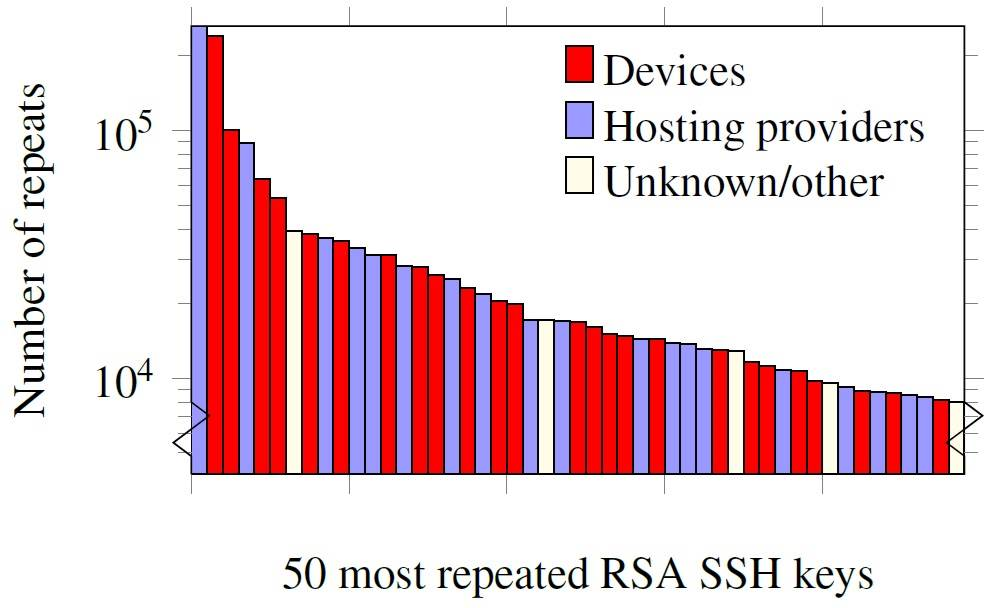
\includegraphics[width=0.5\textwidth]{mining1.jpg}
   \caption{Repeated SSH keys \cite{}}
   \label{fig:IGEDec}
\end{figure}           
      
\subsubsection*{\textbf{Fingerprint key based on Coppersmith's algorithm}}

Coppersmith's algorithm can be applied to factorize modulus $n$ when partial information about $p,q$ or exponent is given. Bernstein factored RSA keys from certified smart cards using Coppersmith's algorithm in \cite{}.
After Bernstein's work, algorithmic flaw in the construction of primes for RSA key generation in a widely-used library of a major manufacturer of cryptographic hardware was found \cite{}. All RSA primes as well as the moduli $n$ generated by RSALib have the	following form: $p=k*M + (65537^a$ mod $M$). The integers $k,a$ are unknown, and RSA primes differ only in their values of $a$ and $k$ for keys of the same size. The major characteristic of the RSA keys is that the size of M is large and almost comparable to the size of the prime p. It causes a significant loss of entropy of resulting RSA primes and then the pool from which primes are randomly generated is reduced. 
       
Matus exploit this vulnerability to factorize $n$. They designed an extension of Coppersmith's factorization attack. This method does not need additional information except modulus $n$ and does not depend on a weak number generator. By extension of Coppersmith's attack, 1024-bit RSA key can be factorized in a feasible time. Table 2 describes an estimation of factorization times for different key lengths on computational devices. Computer 1 is equipped with Intel E5-2650 v3.3GHz Q2.2014 and Computer 2 is equipped with two Intel E5-2666 v3.2.90GHz.

\begin{table}[h]
\centering
\label{my-label}
\begin{tabular}{|c|c|c|}
\hline
Key Size & Computer 1 & Computer 2 \\ \hline
512-bit  & 1.93 CPU hours                                   & 0.63 hours                                                        \\ \hline
1024-bit & 97.1 CPU days                                    & 31.71 days                                                        \\ \hline
2048-bit & 140.8 CPU years                                  & 45.98 years                                                       \\ \hline
\end{tabular}
\caption{An estimation of factorization times for different key lengths on two computational devices \cite{}}
\end{table}



In real world, electronic identity documents (eIDs) domain is significantly affected by the attack. Also it is possible to exploit Trusted Platform Modules (TPMs) with non-negligible probability. Thus, NIST FIPS 140-2 and CC EAL 5+ certified devices are shown to be vulnerable to Coppersmith's attack. 


\section{Evaluation}

\subsection{private key}

\subsubsection{RNG vulnerabilities}
Public key cryptosystem such as RSA, Diffie-Hellman is considered to be secure if properly implemented. However, there are several issues to implement cryptosystem perfectly. In this work, we focused on vulnerabilities of prime number generation process. There are three main weaknesses of RNG in recent works: not avoiding certain prime features, low-entropy problem, and non-uniform distribution of prime. 
Evading certain prime features 

\begin{thebibliography}{9}
\bibitem{a}
Authors, ``Title,'' {\em Journal}, Pages, etc...
\bibitem{b}
Authors, {\em Book title}, Publisher, Year, etc...
\end{thebibliography}

\end{document}
% end of file
